\cleardoublepage
\chapter{The rise of \ebook{}s} \label{ch:intro} % ``Introduction'' is too boring!

\redmarginpar{Note: this chapter is currently pretty much word for word the content of the interim
report, and therefore needs a complete rewrite. I'll update it when the rest is written.}

%\marginpar{Blurb re: portable devices, screen sizes etc}

The recent surge in popularity of devices such as the Amazon Kindle and the Apple iPad has vastly
increased the sale and distribution of \ebook{}s. Amazon.com recently announced\cite{Amazon.com2011}
that during the month of April 2011, Kindle Store sales outstripped print book sales by 105 to 100.
This figure does not include free \ebook{}s `sold' through the Kindle Store, which would skew the
figures significantly further. It was also reported that Amazon's UK Kindle Store, which opened in
September 2010, was, over the same period, outselling hardback books by a factor of two to one.
These ratios are likely to increase as time goes on.

\section{Devices}
\redmarginpar{Amazon\ed kindle apps for PC, iPhone, iPad, netbooks, \emph{actual} kindles\ldots a
plethora
of sizes! Many are battery powered. Don't want to kill the battery, but don't want output to look
crap.}
In addition to dedicated \ebook{} readers, such as the Amazon Kindle and the Sony Reader, many other
devices can be equipped to read the same \ebook{} files, such as tablets, mobile phones, laptops,
netbooks, and desktop PCs. Indeed, virtually every modern device with network connectivity and a
screen can be equipped to read \ebook{}s. Consequently, \ebook{} files are expected to be read on a
wide range of screen sizes and types.

\todo{write something about range of screen sizes/types/pixel densities}

\section{File formats}
Three formats currently dominate the \ebook{} market: \epub{} and Mobipocket, which allow the
document to be formatted to fit the display device, and \gls{pdf}, which does not. Currently there is
no middle ground\ed a document may either be fully rendered to a fixed layout, or completely
unrendered, to be laid out at the mercy of a display device's decisions. Amazon's proprietary Kindle
format is derived from Mobipocket; \gls{pdf} and \epub{} are open standards.

\subsection{PDF}
\gls{pdf} was originally designed as a way of faithfully reproducing documents both on screen and in
print. For this reason, it is almost entirely pre\-s\-en\-ta\-tion-oriented and will not necessarily
include any information on the semantic structure of a given document. The archetypal \gls{pdf}
file consists solely of drawing operators which describe the document pages. There is no
compulsion for these drawing operators to render the page in an order that might be considered
sensible: for example, if a \gls{pdf} generator program decided to render every character on a page in
alphabetical order, or radially outwards from the centre, the resulting file would still be
semantically valid, and the result might well be unnoticeable to the end user. This lack of imposed
semantic structure can make it difficult to infer the best way to `unpick' \gls{pdf} files to allow
their content to be reflowed into a new layout.

This is not to say that \gls{pdf} files \emph{cannot} represent the semantic stucture of their
content\ed indeed as early as 1999, \gls{pdf}~1.3 introduced \emph{logical structure}
facilities\cite{Adobe2001}, adding an optional \emph{structure tree} to the \gls{pdf} specification,
and \emph{tagged \gls{pdf}}, introduced in \gls{pdf}~1.4 in 2001, provides various extensions to this.
Unfortunately, \gls{pdf} documents which actually make good use of these facilities are few and far
between, even a decade after their introduction.

\todo{Mention why tagged \gls{pdf}/structure tree aren't particularly useful for reflow (ie helps
to unpick, but still need to re-typeset... no better off than html)}

\subsection{HTML based}
\label{html-format}
Both \epub{} and Mobipocket are largely based on \html{}. Whilst the use of \xml{}-like formats
allows the semantic structure of documents to be very well defined, in general their presentation
can only be specified in a very loose manner. The user is often presented with a choice of typefaces
and point sizes, essentially allowing the reader software to render the document in any arbitrary
way it chooses. Since an \html{}-derived format has no concrete presentation associated with it,
each time the document is displayed its layout must be recalculated, just as
an interpreted programming language needs to be interpreted each time it runs. (We can therefore
compare \gls{pdf} to a compiled program: it is the result of an optimisation process performed upon
some semantically higher-level representation.) For an \ebook{} reader to maximise its battery life,
this `interpretation' needs to be as simple as possible, \ie{} the algorithm used must not be too
complex, since the more \textsc{cpu} cycles spent executing it, the
less time the \textsc{cpu} can spend idle, and thus the greater the drain on the device's battery.
Furthermore, the longer that is spent formatting the output, the longer the delay between page turns
on the device, and with the speed of \textsc{cpu}s used in these devices ($<$ 500 \textsc{MHz}) it
does not take too large an increase in computation for the page-turn time to become noticeable.



\section{Limitations}



The design paradigm of \gls{pdf}, conceived in the early 1990s\cite{Warnock1991}, was to form a perfect
analogue of the printed page, which would be exactly reproducible regardless of the system on which
the file was rendered. For this reason, it is possible to embed fonts within \gls{pdf} files, to ensure
faithful reproduction on any system, regardless of which fonts are actually installed. In general, a
well typset \gls{pdf} file looks good wherever it is displayed, but, stemming from the `digital sheet
of paper' paradigm, page sizes in a \gls{pdf} document are necessarily fixed at creation-time. An
overwhelming majority of \gls{pdf} documents are rendered for  US letter or A4 size paper. This is fine
if the document is to be printed and read. On a reasonably large screen, the document remains
perfectly readable, and a 10'' netbook or tablet screen may provide acceptable reading. Anything much
smaller (notably mobile phones, and e-readers, such as the Kindle and the Sony Reader) requires
a combination of zooming and panning 
in order to read the document. Documents may, of course, be rendered to a smaller page size, however
the problem still remains\ed it is unlikely that any one page size will be suited to \emph{all}
reading platforms. Most e-readers, using their native (i.e.\ non-\gls{pdf}) formats, allow text to be
resized according to user preference. Indeed, it seems unnecessarily restrictive to force one size
of type upon the user. Of course, paper books suffer from this affliction; digital books need not.
Selling \ebook{}s separately in standard and large-print versions seems perverse when, for virtually
no difference in cost to the publisher/distributor, both can be included in one file. In fact,
if the document is stored at a higher, more abstract level than \gls{pdf}, the text can be rendered
at any desired size, at the cost of the retention of high-quality typesetting afforded by \gls{pdf}.

\marginpar{The rendering engines generally used in e-readers take a \emph{greedy} approach. That is,
they place as many words onto the current line as will fit, and then break, start a new line, and
repeat.}

\epub{} and Mobipocket, both based on \html{}, provide this necessary higher abstraction of
documents. This allows a font size to be specified, and the text to be rendered to closely fit the
screen. Line breaks and page breaks can then be calculated and inserted as necessary, in order to
wrap the text to fit the screen, and to paginate the content. The rendering engines used for
reflowable formats on, e-reader devices, are simplistic\ed but necessarily so. The battery life of
portable devices is lamentably low. Manufacturers of e-readers may claim their products have
batteries which can last for months, but this is principally due to the many shortcuts used when
laying out flowable content. As noted in section~\ref{html-format}, were these devices to use more
complex layout algorithms, which can produce far higher quality typeset output, it would soon emerge
than any savings made by using a low-power electronic paper screen would quickly disappear. In
addition to increasing battery usage, the higher computational complexity of these algorithms may
cause page turns to take longer, as each subsequent page is only rendered when a page turn is
requested. This time delay could be fixed reasonably easily by buffering between page turns, but
this would not solve the battery drain problem.



%\marginpar{Rendering engines are simplistic (but necessarily so, since need to save battery, and not
%take too long per page turn\ed although could buffer between page turns to avoid this) and thus
%don't produce nice results.}




\epub{} allows fonts to be embedded, but Mobipocket does not. Mobipocket files (and by extension,
Kindle files) are therefore restricted to be rendered in a typeface local to (and often chosen by)
the reader software. The Kindle, as an example, provides the user with a choice of `regular',
`condensed', or `sans-serif' for the main body text of its documents. There are bold and italic
variations of these, which are applied according to formatting instructions within the documents
themselves. Additionally, there is a typewriter-style font which document authors may choose to use
in the same manner. The Mobipocket specification supports a very limited subset of \html{} and
\css{}, which makes complex layouts, such as those involving arbitrary indentation or font size
changes, virtually impossible. Figures \ref{alices1} and \ref{alices2} demonstrate the well known
`Mouse's Tale' from Lewis Carroll's \emph{Alice in Wonderland}, in numerous formats.


\begin{figure}[tb]
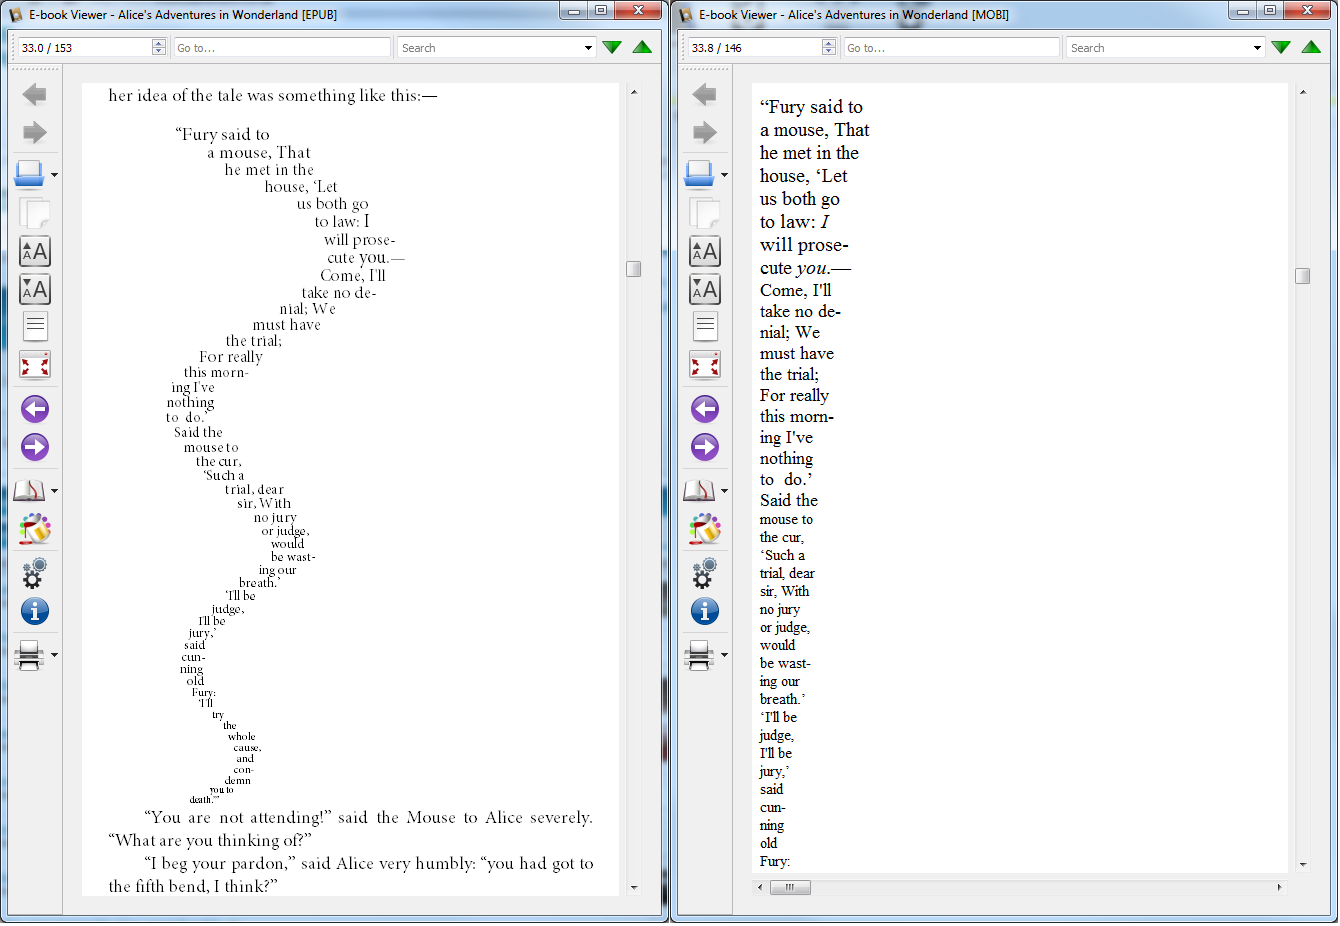
\includegraphics[width=\textwidth]{gfx/alices1}
\caption[Document displayed in Calibre]{On the left is
an \epub{} version of Alice in Wonderland, displayed in Calibre (an open source desktop \ebook{}
viewer). On the right is the same file, converted to Mobipocket, also displayed in Calibre. Note
that in addition to the indentation being lost, the (embedded) font from the \epub{} is no longer
present in the Mobipocket file.}
\label{alices1}
\end{figure}

%\marginpar{Mobipocket\ed can't embed fonts... very limited choice of html to use. Reliant on
%rendering engine of device.
%\epub{}\ed can embed fonts, can style with \css{} pretty much arbitrarily, but still needs to be
%retypeset on each viewing and thus relies on the crappy built in rendering engine of the device.}

\epub{} is a little more flexible, in that it supports a more comprehensive range of \xhtml{} and
\css{}, and allows for arbitrarily complex styling. \epub{} files are still entirely reliant on the
rendering engine of the display device correctly displaying their content, as they have no concrete
layout associated with them.

\begin{figure}[tb]
\begin{center}
\vspace{-.3in}
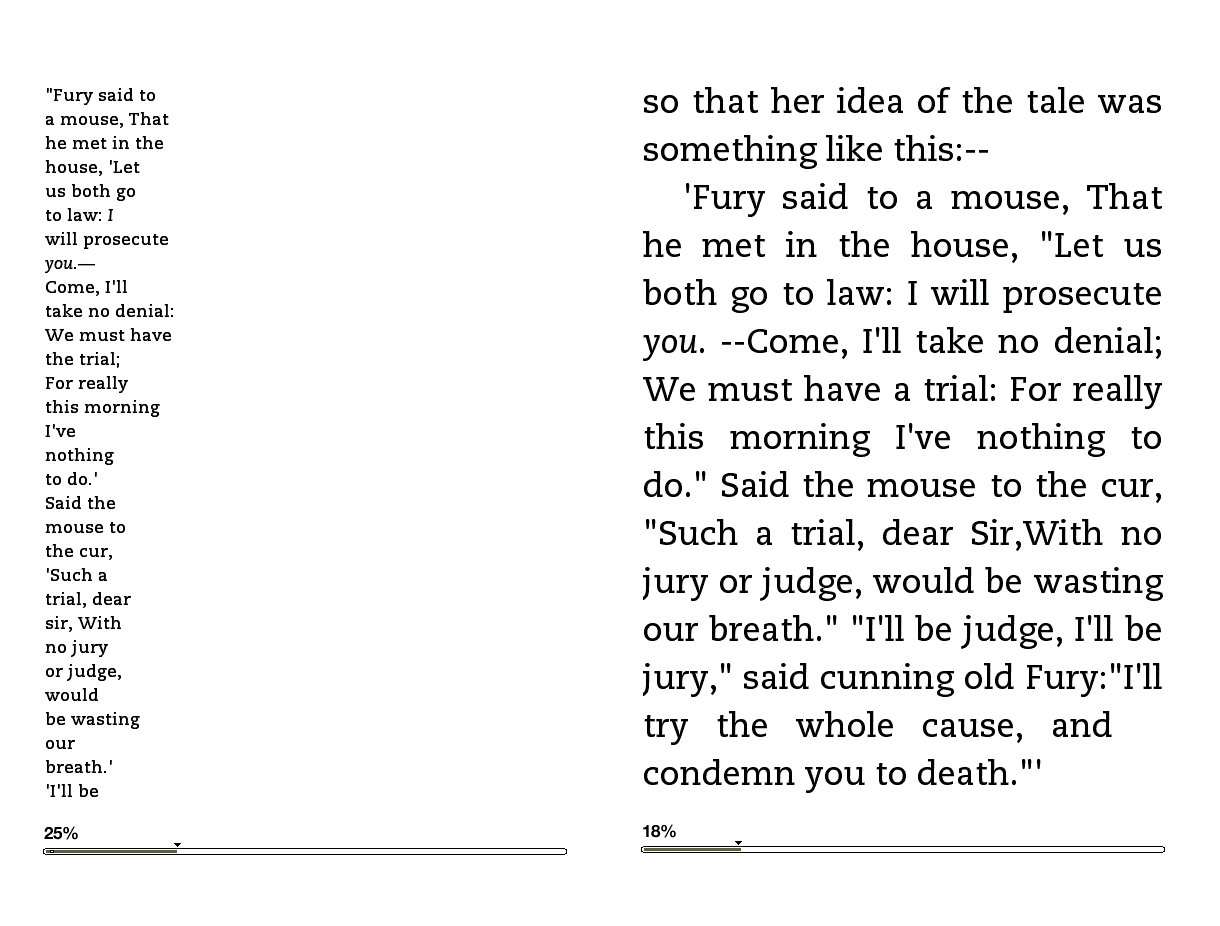
\includegraphics[width=\textwidth]{gfx/alices2}
\end{center}
\vspace{-.3in}
\caption[The same document displayed on the Kindle]{On
the left is the Mobipocket version of Alice in Wonderland (from figure~\ref{alices1}) displayed on
the Kindle. Note that the sizing instructions appear to have been ignored. On the right is the free
version of Alice in Wonderland from the Kindle store, displayed on the Kindle. Note that no attempt
has been made to render the poem in a `tail' shape.}
\label{alices2}
\end{figure}

\section{``Good'' typesetting}
\label{goodtypesetting}
The paper \emph{Reflowable Documents Composed From Pre-rendered Atomic Components}\cite{Pinkney2011}
(attached as an appendix) goes into some detail, particularly in sections 2.1 and 2.2, of what sort
of properties to expect from good-quality typesetting.

\redmarginpar{H+J. What is good H+J? Good hyphenation algorithm. Word spacing. Letter spacing. Glyph
reshaping. Must look at whole paragraph!}

\redmarginpar{Use of kerning. Use of ligatures where appropriate. Avoidance of widows/orphans.}

Knuth and Plass's line breaking algorithm\cite{Knuth1981}, in conjunction with Liang's hyphenation
algorithm\cite{Liang1983}, breaks paragraphs into lines of text to fit a page, resulting in what can be
considered an optimal configuration. \TeX 's default behaviour is then to alter the spacing
between words in order to justify the line to fit the measure of the page. More advanced methods
than simply stretching or shrinking the word spacing do exist, however. Robert Bringhurst, in
\emph{The Elements of Typographic Style}\cite{Bringhurst2008}, suggests that in addition to altering
word spacing, subtle changes to inter-character spacing and individual glyph widths (in the range of
$\pm$ 3\%) can produce more typographically and aesthetically pleasing results. %This is discussed
%further in section~\ref{edgecases}. % no it bloody isn't




